\chapter{Implementación y resultados}
\label{ch:implementacion}

Este capítulo detalla el proceso de construcción del simulador: las decisiones técnicas concretas tomadas en cada componente, los problemas que surgieron durante el desarrollo así como la solución adoptada en cada caso, y los resultados del entrenamiento y evaluación de los modelos de elección modal.

El sistema implementado está disponible como código abierto en \url{https://github.com/ivanuclm/movilidad-urbana}, lo que permite su reproducción, extensión y reutilización en futuros trabajos de investigación, desarrollo o divulgación sobre movilidad urbana. El procedimiento de despliegue para reproducir el entorno local se detalla en el anexo~\ref{anx:despliegue}.


% -------------------------------------------------------
\section{Infraestructura de enrutado viario: OSRM}
\label{sec:impl_osrm}
% -------------------------------------------------------

\subsection{Origen y características del extracto OSM}
\label{subsec:impl_osrm_origen}

Open Source Routing Machine (OSRM) trabaja sobre un extracto de OpenStreetMap (OSM), un fichero binario con extensión \texttt{.osm.pbf} que contiene la geometría de calles, carreteras y caminos de un territorio junto con sus atributos de velocidad, sentido y accesibilidad por modo. Geofabrik \cite{GeofabrikDownloads} distribuye estos extractos por jerarquía geográfica, desde continentes hasta comunidades autónomas.

Se utilizó el extracto de Castilla-La Mancha al ser la región en la que se enmarca el proyecto, escogiendo Toledo como caso de estudio definitivo, tal como se detalla en la sección~\ref{sec:impl_otp}. OpenTripPlanner reutiliza el mismo extracto para la red viaria peatonal, por lo que un único fichero sirve a dos servicios del sistema. La Tabla~\ref{tab:osm_extractos} resume los extractos de OSM evaluados durante el desarrollo.

\begin{table}[H]
  \caption{Comparativa de extractos OSM disponibles en Geofabrik.}
  \label{tab:osm_extractos}
  \centering
  \begin{tabular}{lrl}
    \toprule
    \textbf{Extracto} & \textbf{Tamaño (.osm.pbf)} & \textbf{Uso en el proyecto} \\
    \midrule
    Castilla-La Mancha  & \textasciitilde{}98 MB     & Producción (OSRM y OTP) \\
    % Comunidad Valenciana & \textasciitilde{}131 MB     & Pruebas iniciales con feed EMT Valencia \\
    Comunidad de Madrid & \textasciitilde{}79 MB     & Pruebas con feed EMT Madrid \\
    España              & \textasciitilde{}1{,}3 GB  & Evaluado, descartado por tamaño \\
    Europa              & \textasciitilde{}32{,}0 GB & Descartado por tamaño \\
    \bottomrule
  \end{tabular}
\end{table}

\subsection{Evolución del despliegue}
\label{subsec:impl_osrm_evolucion}

El despliegue de OSRM pasó por tres iteraciones antes de conseguir la configuración definitiva.

\textbf{Fase 1: servidor de demostración oficial.} La primera implementación utilizó el servidor de demostración público del proyecto OSRM (\texttt{router.project-osrm.org}) \cite{OSRMDocs}. Este servidor ofrece acceso gratuito a la API de enrutado sin necesidad de infraestructura local y está pensado para pruebas rápidas de integración. El problema es que solo procesa el perfil de conducción independientemente del indicado en la URL \cite{OSRMIssue4034}; cambiar el perfil en la petición no tiene efecto, lo que hacía inviable la comparación multimodal que el simulador requiere.

\textbf{Fase 2: instancias públicas FOSSGIS.} Las instancias públicas mantenidas por FOSSGIS \cite{FOSSGISRouting} sí devuelven rutas diferenciadas por perfil mediante endpoints independientes (\texttt{/routed-car}, \texttt{/routed-bike}, \texttt{/routed-foot}), lo que permitió confirmar el funcionamiento multimodal y ajustar la integración del backend. El inconveniente es que estos servicios aplican limitaciones de uso (\textit{rate limiting}), presentan latencia variable y no permiten fijar la versión de los datos, lo que compromete la reproducibilidad.

\textbf{Fase 3: instancia local con Docker.} La solución definitiva fue desplegar OSRM localmente mediante la imagen oficial \texttt{osrm/osrm-backend} \cite{OSRMGitHub}, con un contenedor independiente por modo de transporte (conducción, bicicleta y a pie; el transporte público en autobús es responsabilidad de OpenTripPlanner). Esta arquitectura elimina la dependencia de servicios externos en tiempo de ejecución y garantiza reproducibilidad, control de versión y ausencia de límites de cuota. El preprocesado de los grafos, que originalmente se ejecutaba a mano, se automatizó posteriormente como un paso de inicialización de la orquestación Docker Compose (sección~\ref{sec:arch_infra}), de modo que el despliegue completo no requiere ningún comando manual. El procedimiento, tanto automático como los comandos equivalentes paso a paso, se recoge en el anexo~\ref{anx:despliegue}.


\subsection{Pipeline de preprocesado por perfil}
\label{subsec:impl_osrm_pipeline}

Para que OSRM pueda calcular rutas, el extracto \texttt{.osm.pbf} debe transformarse en una estructura de datos interna optimizada para ejecutar consultas y obtener el camino mínimo entre dos puntos del mapa. Este preprocesado se ejecuta una sola vez por perfil y solo hay que repetirlo si se actualiza el extracto de OSM.

Cada perfil define las reglas de movilidad del modo correspondiente: qué tipos de vía son accesibles, a qué velocidad y con qué restricciones de giro. Los tres archivos de perfil estándar (\texttt{car.lua}, \texttt{bicycle.lua} y \texttt{foot.lua}) están incluidos en la imagen oficial de Docker \texttt{osrm/osrm-backend} en \texttt{/opt/}, por lo que no es necesario descargarlos ni configurarlos externamente. Todas las etapas del preprocesado se ejecutan con esa misma imagen, lo que garantiza que el preprocesado sea reproducible en cualquier entorno de ejecución.

\begin{enumerate}
  \item \textbf{Extracción} (\texttt{osrm-extract}): lee el \texttt{.osm.pbf} y construye el grafo viario interno aplicando las reglas del perfil Lua indicado: qué vías son transitables, a qué velocidad y con qué restricciones. El resultado es el fichero \texttt{.osrm} junto con varios auxiliares de índice.
  \item \textbf{Particionado} (\texttt{osrm-partition}): divide el grafo en celdas jerárquicas para el algoritmo Multi-Level Dijkstra (MLD) \cite{Geisberger2008CH}. Esta partición es la que permite calcular rutas de larga distancia en milisegundos, al limitar la búsqueda a fronteras entre celdas en lugar de explorar el grafo completo.
  \item \textbf{Personalización} (\texttt{osrm-customize}): asigna los pesos finales de cada arista sobre la estructura de celdas anterior, produciendo el grafo listo para servir peticiones de ruta.
\end{enumerate}

Las tres etapas generan los ficheros \texttt{clm.osrm} y sus auxiliares, almacenados en directorios separados por perfil (\texttt{osrm-clm/car/}, \texttt{osrm-clm/bike/}, \texttt{osrm-clm/foot/}). Por su tamaño, estos artefactos se versionan mediante Git LFS (\textit{Large File Storage}), una extensión de Git que guarda los ficheros pesados fuera del historial principal y los referencia con punteros ligeros; así un clon del repositorio dispone de los grafos sin necesidad de regenerarlos. El procedimiento completo para reproducirlos se recoge en el anexo~\ref{anx:despliegue}.

El preprocesado completo de los tres perfiles sobre el extracto de Castilla-La Mancha tarda \todo{Revisar tiempos} aproximadamente 97 segundos en la máquina de desarrollo. Los artefactos generados ocupan en total unos 2,1~GB: el perfil de conducción produce 291~MB porque solo incorpora la red viaria accesible al tráfico rodado, mientras que los perfiles de bicicleta y peatonal alcanzan los 911~MB cada uno al incluir además senderos, caminos rurales y zonas de acceso restringido al tráfico.

\begin{figure}[htbp]
  \centering
  % \missingfigure{Diagrama del pipeline de preprocesado OSRM: \texttt{.osm.pbf} $\to$ \texttt{osrm-extract -p \{perfil\}.lua} $\to$ \texttt{osrm-partition} $\to$ \texttt{osrm-customize} $\to$ \texttt{osrm-routed -{}-algorithm mld}. Indicar que el proceso se repite de forma independiente para los tres perfiles (car, bike, foot), generando tres directorios de artefactos separados.}
  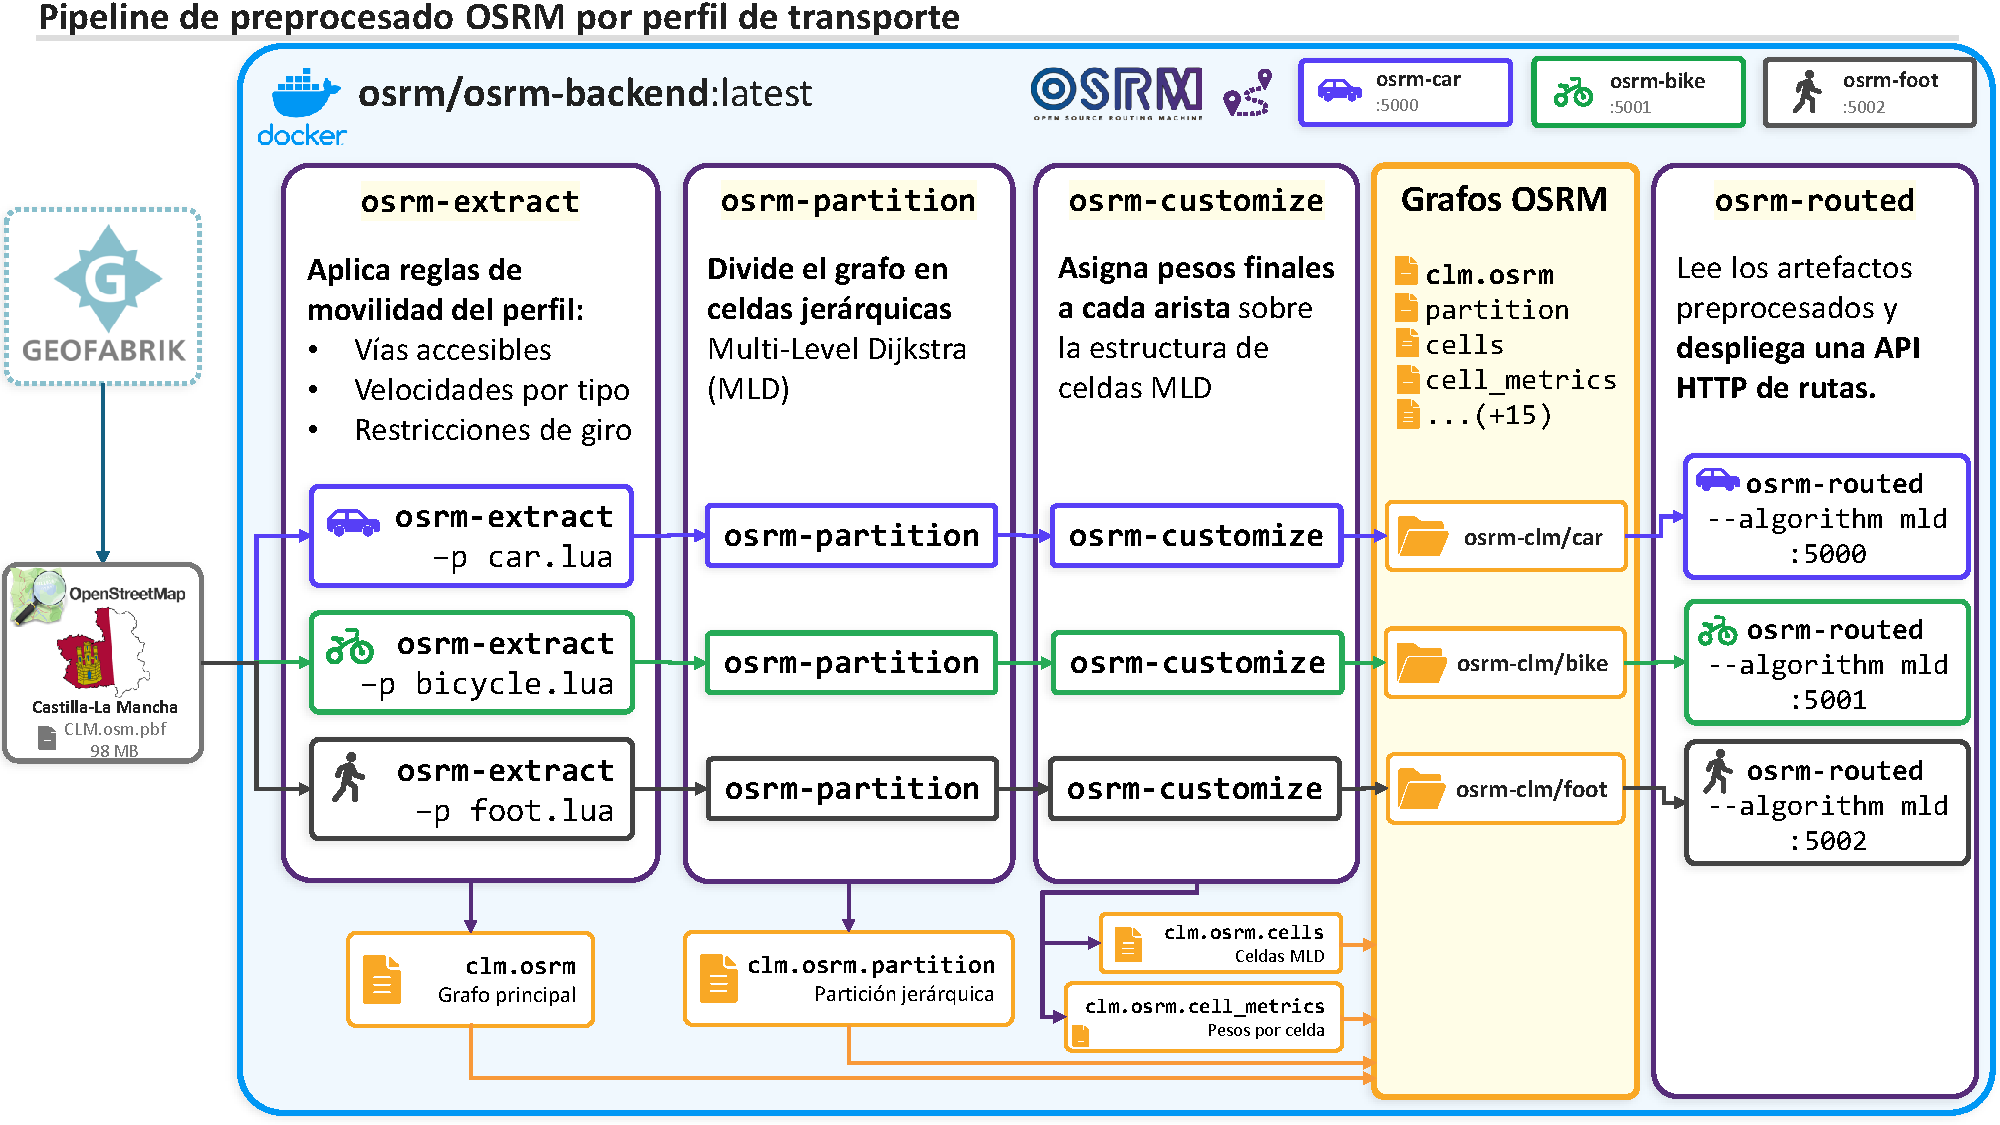
\includegraphics[width=1.0\textwidth]{figs/Pipeline_Preprocesado_OSRM.pdf}

  \caption{Pipeline de preprocesado OSRM por perfil de transporte.}
  \label{fig:osrm_pipeline}
\end{figure}

\subsection{Despliegue y verificación}
\label{subsec:impl_osrm_despliegue}

Cada uno de los tres contenedores OSRM ejecuta el servidor de enrutado sobre su grafo preprocesado con el algoritmo MLD (Figura~\ref{fig:osrm_pipeline}):
\begin{lstlisting}[language=bash]
osrm-routed --algorithm mld /data/clm.osrm
\end{lstlisting}

Los tres contenedores comparten imagen y comando de arranque. Cada uno monta el directorio de artefactos de su perfil (\texttt{osrm-clm/car}, \texttt{osrm-clm/bike}, \texttt{osrm-clm/foot}). Dentro de la red interna de Docker Compose, el proceso \texttt{osrm-routed} escucha siempre en el puerto 5000 en todos los contenedores, y el backend los referencia por nombre de servicio (\texttt{osrm-car}, \texttt{osrm-bike}, \texttt{osrm-foot}) en ese mismo puerto. Para verificar las instancias directamente desde el terminal del anfitrión, cada contenedor expone un puerto distinto hacia el exterior: 5001, 5002 y 5003, respectivamente para los perfiles de conducción, bicicleta y a pie. Se evita el puerto 5000 en el anfitrión porque en macOS lo ocupa por defecto un servicio del sistema (el receptor AirPlay), lo que impediría el arranque del contenedor; esta publicación de puertos solo se usa para depuración, ya que el backend se comunica con OSRM por la red interna.


Una respuesta válida devuelve \texttt{"code": "Ok"} junto con la distancia en metros, la duración en segundos y la geometría en formato polilínea~\cite{GooglePolyline}, una cadena de texto con la secuencia de coordenadas de la ruta, que el backend decodifica antes de enviarla al frontend. Si el grafo está incompleto o el perfil es incorrecto, OSRM devuelve \texttt{"code": "NoRoute"} o una ruta degradada, detectable al comparar visualmente los tres trazados en la interfaz.

\begin{code}[H]
\begin{lstlisting}[language=bash]
# osrm-car  (conduccion, localhost:5001)
curl "http://localhost:5001/route/v1/driving/-4.0356,39.8750;-4.0023,39.8602?overview=full"
# osrm-bike (bicicleta,  localhost:5002)
curl "http://localhost:5002/route/v1/cycling/-4.0356,39.8750;-4.0023,39.8602?overview=full"
# osrm-foot (peatonal,   localhost:5003)
curl "http://localhost:5003/route/v1/foot/-4.0356,39.8750;-4.0023,39.8602?overview=full"
\end{lstlisting}
\caption{Verificación de las tres instancias OSRM desde el terminal del anfitrión. El parámetro \texttt{overview=full} fuerza la devolución de la geometría completa de la ruta; sin él, OSRM devuelve una versión simplificada con menos puntos.}
\label{cod:osrm_verificacion}
\end{code}

La Figura~\ref{fig:osrm_rutas} muestra las tres rutas calculadas simultáneamente para el mismo par origen-destino: en azul, la ruta de conducción sigue las calles principales; en verde, la ruta de bicicleta prioriza carriles bici y calles tranquilas; en gris con línea discontinua, la ruta peatonal puede acceder a zonas restringidas al tráfico rodado. Los tres trazados ponen de manifiesto las distintas restricciones de cada perfil sobre la red viaria de Toledo.

\begin{figure}[H]
  \centering
  \includegraphics[width=1.0\textwidth]{figs/RutasSoloOSRM.jpeg}
  \caption{Rutas OSRM para los tres perfiles de transporte sobre Toledo.}
  \label{fig:osrm_rutas}
\end{figure}

% -------------------------------------------------------
\section{Planificación multimodal: OpenTripPlanner}
\label{sec:impl_otp}
% -------------------------------------------------------

\subsection{Fuente de datos GTFS y proceso de selección}
\label{subsec:impl_otp_gtfs}

OpenTripPlanner requiere dos fuentes de datos: un extracto viario OSM para modelar los tramos de acceso a pie, y un feed GTFS con el servicio programado del operador de transporte público para los tramos en vehículo. Al enmarcarse el proyecto en Castilla-La Mancha, la búsqueda de feed GTFS de bus urbano se orientó a la región desde el principio, con la ventaja de que el extracto OSM ya estaba disponible por su uso en OSRM (sección~\ref{subsec:impl_osrm_origen}). La fuente empleada fue el Punto de Acceso Nacional de Transporte Multimodal (NAP), gestionado por el Ministerio de Transportes y Movilidad Sostenible, que centraliza feeds GTFS de operadores de toda España \cite{NAPHome}. Aunque su cobertura a nivel nacional es amplia, la disponibilidad de feeds de transporte urbano en Castilla-La Mancha resultó muy limitada, como se detalla a continuación.

Las opciones disponibles en Castilla-La Mancha resultaron ser muy escasas. En Albacete solo figuraban servicios de operadores interurbanos como Alsa, sin datos de red urbana en el NAP. Guadalajara contaba con feeds del Consorcio de Transportes de Madrid (cercanías y autobuses interurbanos de la Comunidad de Madrid), pero sin red municipal propia. Cuenca tampoco disponía de feed urbano. La única opción urbana era Ciudad Real, cuyo feed, operado por AISA, incluía también Seseña, con paradas repartidas entre dos localidades separadas por más de 170~km; además, en ese momento no incluía geometría de rutas, requisito imprescindible para la representación cartográfica del servicio.

Ante la ausencia de un feed GTFS de Castilla-La Mancha válido, se evaluaron feeds de otras ciudades como candidatos alternativos para el proyecto. La EMT de Madrid \cite{NAPEMTMadrid}, con 4.914 paradas, 236 rutas y 87.137 viajes programados, sirvió de banco de pruebas para validar la integración de OTP con datos reales y desarrollar los endpoints de la capa estática del backend. El volumen del feed reveló además un problema de paginación: la API, que exige un límite explícito, devolvía solo las primeras 500 paradas por defecto, dejando la red visualmente incompleta. El límite se ajustó a 5.000, suficiente para Madrid y los feeds posteriores.

El feed GTFS elegido finalmente fue el de los autobuses urbanos de Toledo \cite{NAPToledoUrbano}. Con 268 paradas, 56 rutas y 87.751 viajes que cubren unos tres meses de servicio programado, tiene un tamaño ajustado al alcance del simulador, cubre el casco urbano, el polígono industrial y las urbanizaciones periféricas, e incluye geometría de rutas para su representación cartográfica. Como el feed no incluye tarifas, el coste del billete se introduce como parámetro en el panel lateral de la interfaz (de forma que pueda ser fijado por el analista en la simulación), junto al resto de variables del perfil de viajero, para su uso en la inferencia modal.
% El extracto OSM de Castilla-La Mancha ya disponible para OSRM servía también como base viaria para OTP, por lo que no fue necesario descargar ni preprocesar ningún fichero adicional.

\subsection{Periodo de validez del feed y selección de fecha}
\label{subsec:impl_otp_fecha}

Los feeds GTFS del NAP tienen un periodo de validez limitado; para el operador de Toledo (\texttt{GTFS\_Urbano\_Toledo\_2026}), los ficheros publicados cubren del 22 de febrero al 22 de mayo de 2026. Si la fecha de consulta cae fuera de ese rango, OTP no devuelve itinerarios de transporte público y el simulador queda sin oferta de bus sobre la que inferir. Durante el desarrollo se descargaron varias versiones del feed; en las primeras el operador figuraba como ``Autobuses urbanos Toledo'' y en posteriores había pasado a denominarse UNAUTO S.L. (Grupo Ruiz), aunque el formato de los ficheros GTFS se mantuvo en todas las versiones.

El mismo feed alimenta los dos subsistemas que consumen GTFS: el grafo de OTP (sección~\ref{subsec:impl_otp_grafo}) y la capa estática de horarios (sección~\ref{sec:impl_gtfs}), de modo que ambos comparten exactamente la misma ventana de validez. La fecha y la hora de consulta no se fijan en el código: se exponen mediante un control global en la interfaz, con un valor por defecto dentro del rango (\texttt{2026-05-21}, \texttt{12:00}) y acotado al intervalo válido del feed. Al ser un parámetro transversal a toda la simulación, este control único gobierna a la vez los itinerarios multimodales, los horarios de la red y el día y la hora del perfil de inferencia, evitando configuraciones contradictorias entre las distintas vistas; su ubicación y comportamiento en la interfaz se describen en la sección~\ref{subsec:impl_frontend_mapa}. El backend recibe la fecha y la hora en la petición y las traslada a OTP; cuando no se indican, aplica el valor por defecto.

Se fijó la hora por defecto a las 12:00 ya que se sitúa en la franja de mayor frecuencia de servicio y evita el horario nocturno, donde la oferta es reducida o inexistente.

OTP devuelve los instantes de paso en tiempo universal (epoch UTC) acompañados del desfase horario de la agencia (\texttt{agencyTimeZoneOffset}). El backend suma ese desfase antes de formatear las horas, de modo que los itinerarios se muestran en hora local de Toledo (Europe/Madrid), con el horario de verano resuelto automáticamente según la fecha consultada.

\subsection{Construcción del grafo multimodal}
\label{subsec:impl_otp_grafo}

El grafo se construye con un único comando Docker ejecutado sobre el directorio \texttt{otp-toledo/}, que debe contener el extracto OSM (\texttt{clm.osm.pbf}) y el feed GTFS (\texttt{GTFS\_Urbano\_Toledo\_2026.zip}):

\begin{lstlisting}[language=bash]
docker run --rm -v "otp-toledo:/var/opentripplanner" opentripplanner/opentripplanner:2.5.0 --build --save
\end{lstlisting}

OTP lee ambos ficheros y serializa el resultado en \texttt{graph.obj}: la red viaria OSM modela los tramos de acceso a pie a las paradas, y el feed GTFS aporta el servicio programado con horarios, paradas y geometría de las líneas. El proceso tarda unos minutos \todo{tiempos} y solo es necesario repetirlo cuando se actualiza el feed; el extracto OSM puede reutilizarse entre versiones. El comando anterior corresponde a la generación manual del grafo.

% Al igual que los grafos OSRM, el \texttt{graph.obj} no se versiona en el repositorio por su tamaño y debe generarse antes del primer despliegue.\todo{Completar anexo de despliegue con construcción del grafo OTP: comando --build --save y requisitos previos (OSM + GTFS)} Una vez disponible, OTP se lanza en modo de explotación (\texttt{--load --serve}) y queda accesible en el puerto 8080, exponiendo la API REST de planificación \cite{OTPRouteRequest}.

El \texttt{graph.obj} resultante (unos 120\,MB) se versiona mediante Git LFS para que el sistema arranque sin reconstrucción en un clon limpio. Como salvavidas, la orquestación incluye un servicio de inicialización idempotente (\texttt{otp-build}) que ejecuta \texttt{-{}-build -{}-save} únicamente si el grafo no está presente, de forma análoga a la compilación de los grafos OSRM. Una vez disponible, OTP se lanza en modo de explotación (\texttt{-{}-load -{}-serve}) y queda accesible en el puerto 8080, exponiendo la API REST de planificación \cite{OTPDocs}.



\subsection{Integración de itinerarios en el backend}
\label{subsec:impl_otp_integracion}

El router \texttt{/api/otp} del backend consulta OTP mediante peticiones HTTP a \texttt{/otp/routers/default/plan} y deserializa la respuesta para extraer los tramos (\textit{legs}) del itinerario seleccionado. OTP devuelve hasta cinco itinerarios alternativos. El criterio de selección automática es el siguiente: se elige el primero que incluya al menos un tramo de transporte público (modo distinto de \texttt{WALK}); si ninguno cumple esta condición, se devuelve el de menor duración total. El frontend permite paginar entre las alternativas mediante los botones ``Anterior'' y ``Siguiente'', que transmiten el índice del itinerario deseado al backend, garantizando que el vector de características para la inferencia se calcula siempre sobre el mismo itinerario que se visualiza.

Para cada tramo del itinerario seleccionado se devuelve: modo de transporte, distancia, duración, geometría decodificada, parada de inicio y fin, nombre de línea, agencia y horarios de salida y llegada en formato \texttt{HH:MM}. Para los tramos de transporte público se añade a la consulta el parámetro \texttt{showIntermediateStops}, que incorpora a la respuesta de OTP las paradas intermedias de cada tramo; con ellas el backend compone la secuencia ordenada completa de paradas del tramo, desde el embarque hasta el desembarque, anotando para cada una su nombre, coordenadas y hora de paso. Esta secuencia alimenta el diagrama de paradas del itinerario descrito en la sección~\ref{subsec:impl_frontend_legs}. La geometría, codificada en formato polyline, se decodifica en el frontend y se concatena para componer la traza completa del itinerario.


Cuando la distancia entre origen y destino es muy corta, o cuando no existe servicio de autobús entre los dos puntos en el horario fijado, OTP puede devolver como mejor itinerario una ruta completamente a pie, equivalente en tiempo y trayecto a la que ya proporciona OSRM con el perfil peatonal. En ese caso, si se construyese el vector de características de transporte público con los valores devueltos (tiempo de acceso cero, tiempo en bus cero, transbordos cero), el modelo podría asignar una probabilidad elevada al transporte público en trayectos sin servicio real. La solución adoptada, descrita en la sección~\ref{subsec:impl_backend_penalizacion}, consiste en detectar esta situación y sobrescribir las características de transporte público del vector con valores de penalización que llevan al modelo a descartar ese modo.

La Figura~\ref{fig:otp_itinerario} ilustra un itinerario multimodal típico en la interfaz del simulador: un tramo a pie inicial (trazado discontinuo en tono naranja oscuro) conecta el origen con la parada de embarque, un tramo en autobús (trazado continuo del color de la línea) cubre el recorrido principal, y un tramo a pie final lleva hasta el destino; las paradas del trayecto se marcan sobre el mapa con el color de su línea. En el panel lateral, una cabecera resume las horas de salida y llegada y la duración total, y bajo ella se despliega el detalle tramo a tramo: los tramos a pie como una línea de resumen y cada tramo en autobús como un diagrama vertical con todas sus paradas y la hora de paso por cada una. Al pulsar una parada del diagrama, el mapa se centra en ella y muestra su información, y los transbordos entre líneas se señalan de forma explícita.


\begin{figure}[H]
  \centering
%   \missingfigure{Captura de la interfaz mostrando un itinerario multimodal OTP sobre el mapa de Toledo: tramo a pie inicial (línea discontinua gris) desde el origen hasta la parada de embarque, tramo en autobús (línea continua de color) y tramo a pie final hasta el destino. En el panel lateral, desglose del itinerario con cada leg: modo, duración en minutos, paradas de inicio y fin, nombre de línea y horario de salida.}
    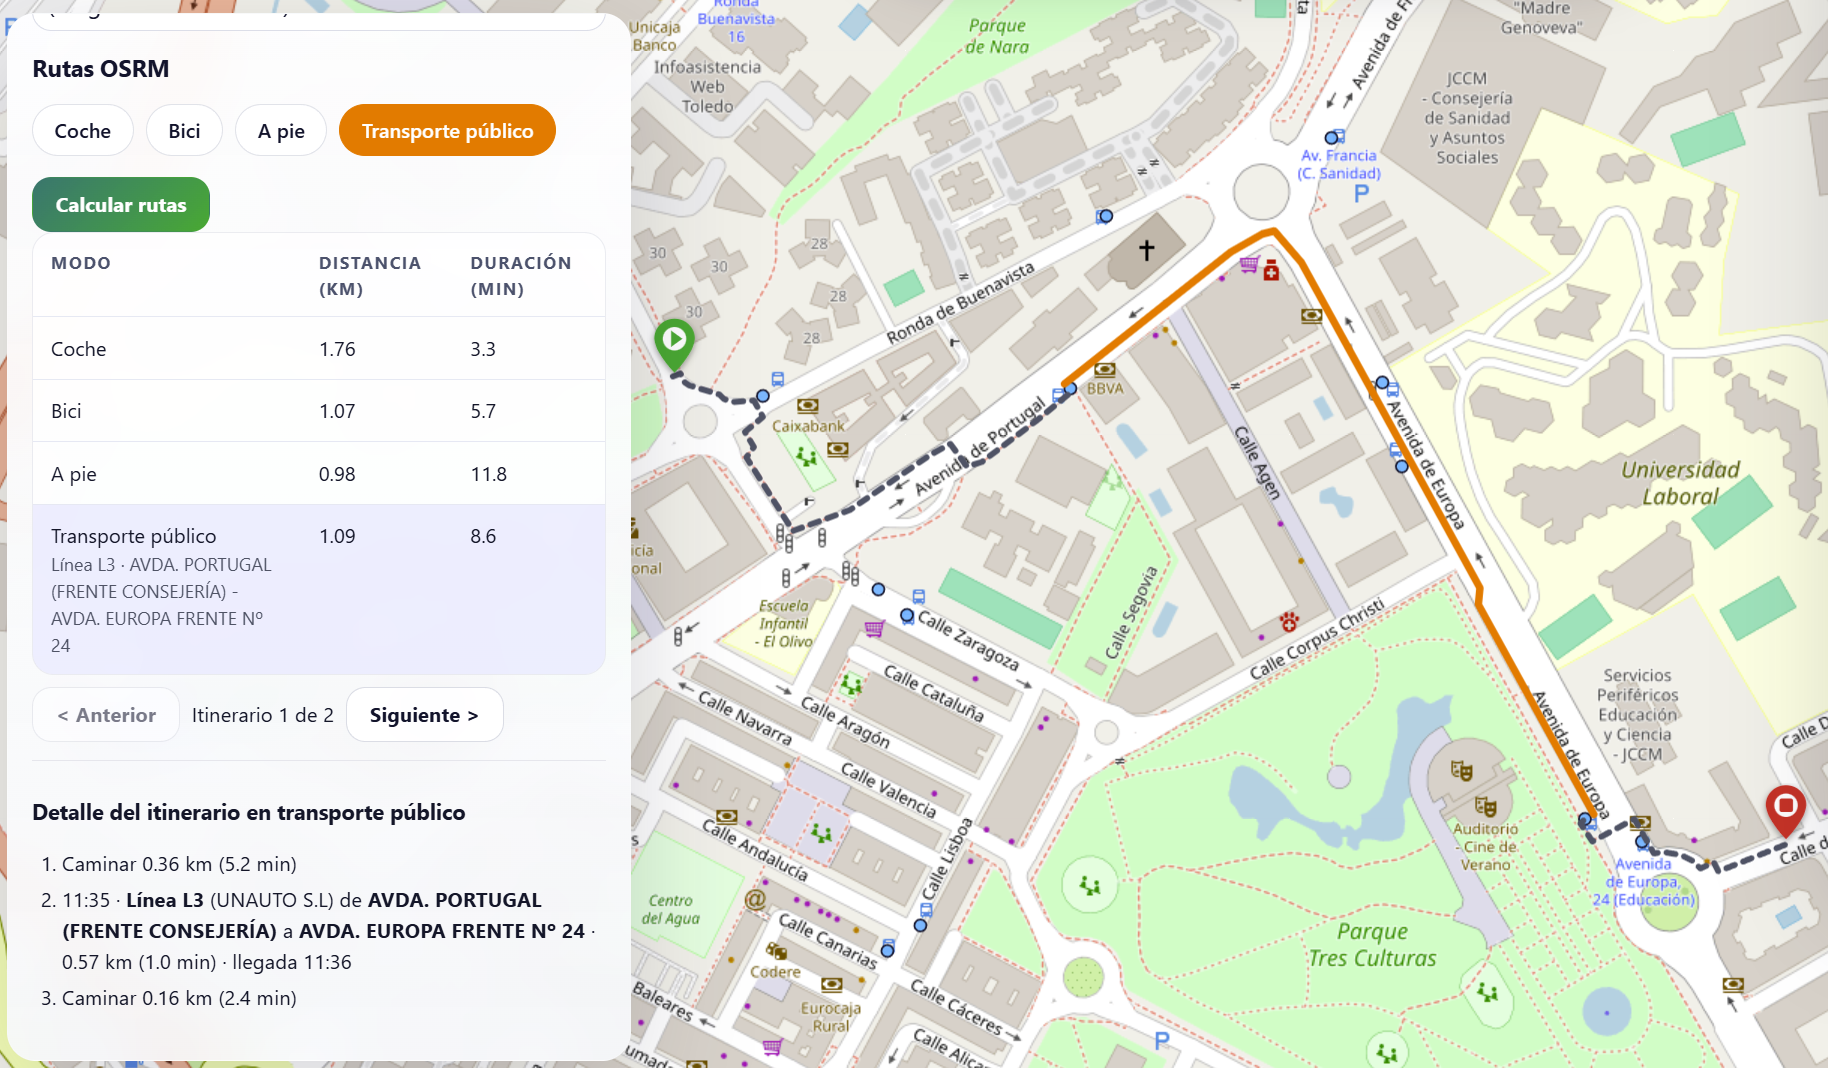
\includegraphics[width=1.0\textwidth]{figs/ItinerarioMultimodalZoom.png}
  \caption{Itinerario multimodal OTP con desglose de tramos en la interfaz.}
  \label{fig:otp_itinerario}
\end{figure}

% -------------------------------------------------------
\section{Integración del feed GTFS}
\label{sec:impl_gtfs}
% -------------------------------------------------------

\subsection{Arquitectura de la capa estática}
\label{subsec:impl_gtfs_arquitectura}

El router \texttt{/api/gtfs} expone la información estática de la red de autobús directamente a partir de los ficheros del feed GTFS, sin depender de OpenTripPlanner. Esto permite consultar y visualizar la red (paradas, líneas y horarios) de forma independiente del planificador.


El feed GTFS consiste en una colección de archivos de texto plano con extensión \texttt{.txt} y formato de valores separados por comas, empaquetados en un único archivo ZIP \cite{GTFSOverview}. En el arranque del servicio, el backend descomprime y carga en memoria con \texttt{pandas} los seis ficheros necesarios: \texttt{stops.txt} (paradas con coordenadas y nombre), \texttt{routes.txt} (líneas de la red), \texttt{trips.txt} (servicios programados por línea), \texttt{stop\_times.txt} (horarios de paso por cada parada), \texttt{shapes.txt} (geometría de los trazados) y \texttt{calendar\_dates.txt} (calendario de excepciones de servicio) \cite{GTFSReference}. Los DataFrames resultantes permanecen en memoria durante toda la vida del proceso.


Responder a preguntas como ``¿qué líneas pasan por esta parada?'' o ``¿cuál es el horario de una ruta para una fecha concreta?'' requiere cruzar varios de estos ficheros, tal como ilustra la Figura~\ref{fig:gtfs_joins}. Para obtener las líneas asociadas a una parada se encadenan tres cruces: \texttt{stops.txt} $\to$ \texttt{stop\_times.txt} $\to$ \texttt{trips.txt} $\to$ \texttt{routes.txt}. Para los horarios por fecha se añade el filtro de \texttt{calendar\_dates.txt}, que indica los días en que cada servicio está activo. Mantener todos los ficheros en memoria evita releer el feed completo en cada petición y elimina la necesidad de añadir una base de datos para datos que no cambian en tiempo de ejecución.

\begin{figure}[htbp]
  \centering
  \missingfigure{Diagrama de los seis ficheros GTFS como cajas (\texttt{stops}, \texttt{stop\_times}, \texttt{trips}, \texttt{routes}, \texttt{shapes}, \texttt{calendar\_dates}) con flechas que muestran los cruces por clave: \texttt{stops}\,--\,\texttt{stop\_times} (stop\_id), \texttt{stop\_times}\,--\,\texttt{trips} (trip\_id), \texttt{trips}\,--\,\texttt{routes} (route\_id), \texttt{trips}\,--\,\texttt{shapes} (shape\_id) y \texttt{trips}\,--\,\texttt{calendar\_dates} (service\_id). Resaltar la cadena stops$\to$stop\_times$\to$trips$\to$routes que resuelve ``líneas por parada''.}
  \caption{Cruces entre los ficheros del feed GTFS para resolver las consultas de la capa estática.}
  \label{fig:gtfs_joins}
\end{figure}

\subsection{Endpoints disponibles}
\label{subsec:impl_gtfs_endpoints}

La capa GTFS expone cuatro endpoints que cubren las operaciones necesarias para la visualización cartográfica y la consulta de la red:

\begin{itemize}
   \item \textbf{Listado de paradas} (\texttt{GET /api/gtfs/stops}): devuelve todas las paradas del feed con identificador, nombre, coordenadas y líneas asociadas. Acepta un parámetro \texttt{limit} (5.000 por defecto, suficiente para el feed de Toledo con 268 paradas) y un filtro de bounding box opcional para restringir el resultado al área visible en el mapa.

  \item \textbf{Listado de rutas} (\texttt{GET /api/gtfs/routes}): catálogo completo de líneas con identificador, nombre corto, nombre largo y atributos de color cuando están disponibles en el feed.

  \item \textbf{Detalle de ruta} (\texttt{GET /api/gtfs/routes/\{route\_id\}}): dado el identificador de una línea, devuelve la secuencia ordenada de paradas y la geometría del \textit{shape} asociado para su representación cartográfica.

\item \textbf{Horarios por fecha} (\texttt{GET /api/gtfs/routes/\{route\_id\}/schedule}): dado un identificador de ruta y una fecha especificada mediante el parámetro de consulta \texttt{date} (es decir, \texttt{?date=YYYY-MM-DD}), devuelve los servicios programados agrupados por dirección, con primera y última salida y listado completo de horarios. Al igual que con OTP (sección~\ref{subsec:impl_otp_fecha}), la interfaz usa una fecha fija dentro del rango de validez del feed en lugar de la fecha del sistema. Cualquier fecha posterior al rango de validez devuelve cero servicios.
\end{itemize}


\subsection{Coloración de líneas y agrupación por sentido}
\label{subsec:impl_gtfs_color}

El feed GTFS de Toledo incluye en \texttt{routes.txt} un color por línea (campos \texttt{route\_color} y \texttt{route\_text\_color}), que la interfaz utiliza directamente para mostrar cada línea con el color oficial del operador. Si un feed no incluye esos campos, la función \texttt{routeColor()} genera un color de reserva a partir del nombre corto de la línea: transforma el texto en un número entero y lo reduce módulo 360 para elegir un tono; la saturación y la luminosidad se mantienen fijas (70\,\% y 35\,\%, respectivamente) para que el color resultante tenga siempre contraste suficiente con el texto blanco superpuesto. Como un mismo nombre produce siempre el mismo número, cada línea conserva su color entre ejecuciones. El Código~\ref{cod:gtfs_color} recoge ambas funciones.

\begin{lstlisting}[language=Java, caption={Color de línea: feed GTFS como fuente primaria y hash determinista como respaldo.}, label={cod:gtfs_color}]
function hslForKey(key: string): string {
  let h = 0;
  for (let i = 0; i < key.length; i++) h = (h * 31 + key.charCodeAt(i)) | 0;
  return `hsl(${Math.abs(h) % 360}, 70%, 35%)`;
}
function routeColor(r: { color?: string | null; short_name?: string | null; id: string }): string {
  if (r.color) return `#${r.color}`;
  return hslForKey(r.short_name || r.id);
}
\end{lstlisting}

Este criterio de color se aplica de forma homogénea en toda la interfaz: en las etiquetas de línea del catálogo y del panel de rutas, en las etiquetas de las paradas, en el diagrama de paradas y en el trazado de la línea sobre el mapa. Algunas líneas del feed de Toledo son de color blanco (por ejemplo, la L14), y parecería invisible sobre el fondo claro de los paneles y del mapa. Para evitarlo, la función \texttt{isLightColor()} mide cuán claro es un color a partir de sus componentes de rojo, verde y azul y, si supera un umbral cercano al blanco, le añade un contorno oscuro.

El feed de Toledo contiene 56 entradas en \texttt{routes.txt} pero solo 25 líneas distintas, ya que el operador registra cada sentido y variante de recorrido como un \texttt{route\_id} independiente con el mismo \texttt{route\_short\_name}. La interfaz agrupa esas entradas por nombre corto en un diccionario (\texttt{routeSiblingsByShortName}), de modo que el catálogo muestra una sola entrada por línea. Cuando el usuario selecciona una línea, el sentido activo se deduce de la posición del \texttt{route\_id} elegido dentro del grupo de variantes; así, al pulsar la etiqueta de una parada en el mapa (que conoce el \texttt{route\_id} exacto del servicio que pasa por ella) se activa directamente el sentido correcto, sin lógica adicional.

La Figura~\ref{fig:gtfs_paradas} muestra el panel Red GTFS. El catálogo se organiza en un acordeón donde cada fila representa una línea física con su badge coloreado y nombre largo. Al expandir una entrada con varios sentidos, aparece una sublista con las variantes (sentidos) de la línea y el identificador activo resaltado mediante un borde lateral de su color. El panel muestra además un diagrama vertical de paradas inspirado en los paneles de andén: una barra vertical del color de la línea, con las terminales como puntos rellenos, las paradas intermedias como aros huecos y la parada de referencia resaltada en azul. Al pulsar sobre el nombre de una parada, el mapa ejecuta un desplazamiento animado (\texttt{flyTo}) hasta esa posición. Una tabla de salidas agrupada por hora completa la información de la ruta seleccionada; las salidas se muestran siempre para la fecha activa, atenuando las anteriores a la hora seleccionada en el control global, resaltando en azul las posteriores y en negrita la próxima salida. Si la línea no circula el día elegido, se sustituye la tabla por un aviso que indica los días en que sí presta servicio. De este modo el panel no necesita sus propios selectores de día: la fecha y la hora provienen del control global descrito en la sección~\ref{subsec:impl_otp_fecha}.



\begin{figure}[H]
  \centering
  \missingfigure{Panel Red GTFS: a la izquierda, el acordeón con la línea seleccionada desplegada mostrando el diagrama vertical de paradas y la tabla de horarios agrupada por hora (con las salidas pasadas atenuadas y la próxima resaltada); a la derecha, el trazado de la línea sobre el mapa de Toledo con sus paradas coloreadas.}
  \caption{Panel GTFS con acordeón de líneas, diagrama de paradas y horarios.}
  \label{fig:gtfs_paradas}
\end{figure}

% -------------------------------------------------------
\section{Implementación del backend FastAPI}
\label{sec:impl_backend}
% -------------------------------------------------------

\subsection{Estructura modular}
\label{subsec:impl_backend_estructura}

El backend está implementado con FastAPI sobre Python y organizado en módulos por responsabilidad. Un directorio \texttt{api/} contiene los cuatro routers (\texttt{routes\_osrm.py}, \texttt{routes\_otp.py}, \texttt{routes\_gtfs.py}, \texttt{routes\_lpmc.py}); un directorio \texttt{services/} contiene la lógica de negocio desacoplada de la capa HTTP (\texttt{osrm\_client.py}, \texttt{lpmc\_inference.py}); y el módulo raíz \texttt{main.py} monta los routers y habilita CORS (\textit{Cross-Origin Resource Sharing}), el mecanismo que autoriza al navegador a que la interfaz web, servida desde un puerto distinto, consuma la API del backend. Los endpoints expuestos por cada router se recogen en la Tabla~\ref{tab:endpoints_api} del capítulo~\ref{ch:arquitectura}.

La separación en módulos permite desarrollar, probar y documentar cada router de forma independiente. FastAPI genera documentación OpenAPI automática en \texttt{/docs} que refleja el estado actual de los endpoints en tiempo real, lo que facilitó la verificación del contrato de cada integración durante el desarrollo sin necesidad de un cliente HTTP externo.

\begin{figure}[htbp]
  \centering
  \missingfigure{Captura de la documentación OpenAPI automática (\texttt{/docs}) del backend FastAPI, mostrando los cuatro grupos de endpoints (/api/osrm, /api/otp, /api/gtfs, /api/lpmc) con sus rutas, métodos HTTP y esquemas de petición y respuesta.}
  \caption{Documentación OpenAPI generada automáticamente por FastAPI.}
  \label{fig:fastapi_docs}
\end{figure}

\subsection{Router OSRM: consultas multiperfil}
\label{subsec:impl_backend_osrm}

El router \texttt{/api/osrm/routes} acepta un par origen-destino y una lista de perfiles solicitados, y lanza las consultas a los tres contenedores OSRM en paralelo mediante \texttt{asyncio.gather}. La paralelización reduce la latencia total al tiempo de la consulta más lenta en lugar de la suma de las tres, lo que es especialmente útil cuando se solicitan los tres perfiles a la vez. Para cada perfil, el backend recibe la distancia en metros, la duración en segundos y la geometría en formato polyline, decodifica esta última en una lista de coordenadas \texttt{[lat, lon]} lista para Leaflet, y convierte las duraciones de segundos a horas antes de construir el vector de características, ya que el dataset LPMC almacena todas las duraciones en esa unidad.

\subsection{Router OTP: itinerarios multimodales}
\label{subsec:impl_backend_otp}

El router \texttt{/api/otp/routes} consulta el endpoint de planificación de OTP, gestiona la selección de itinerario (automática o por índice explícito recibido desde el frontend) y transforma la respuesta de OTP a un formato propio y homogéneo de tramos, más sencillo de consumir por el frontend. Para cada tramo del itinerario seleccionado se devuelve: modo de transporte, distancia, duración, geometría decodificada desde polyline, parada de inicio y fin, nombre de línea, agencia y horarios de salida y llegada. La geometría de cada tramo se concatena para formar la traza completa del itinerario, que el frontend divide y renderiza por segmentos según el modo.

\subsection{Penalización de itinerarios sin transporte público real}
\label{subsec:impl_backend_penalizacion}

Cuando OTP devuelve un itinerario compuesto exclusivamente por un tramo a pie, sin ningún tramo de transporte público, las características de transporte público del vector de entrada (tiempo de acceso a la parada, tiempo en el vehículo, tiempo de espera y de transbordo, y número de transbordos) tomarían valores próximos a cero. El problema es que esos mismos valores bajos caracterizan en el dataset a un transporte público rápido y directo, por lo que el modelo podría asignar una probabilidad elevada al transporte público en un trayecto donde en realidad no hay servicio. El caso se detectó durante las pruebas de integración del módulo de inferencia: en trayectos cortos en los que la opción más rápida era ir a pie, OTP devolvía ese único tramo como mejor itinerario y la inferencia resultaba engañosa.

Para evitarlo, el backend comprueba si el itinerario contiene algún tramo de transporte público. Si no es así, sobrescribe las seis características de transporte público (\texttt{dur\_pt\_access}, \texttt{dur\_pt\_bus}, \texttt{dur\_pt\_rail}, \texttt{dur\_pt\_int\_waiting}, \texttt{dur\_pt\_int\_walking} y \texttt{pt\_n\_interchanges}) con un valor situado en el extremo superior de su distribución. En concreto, a cada característica se le asigna el valor que, tras el escalado estándar (\texttt{StandardScaler}) del modelo, queda cinco desviaciones típicas por encima de la media de entrenamiento: es decir, $\mu + 5\sigma$, tomando la media $\mu$ y la desviación típica $\sigma$ que el escalador aprendió de esa característica. De este modo el modelo percibe un transporte público con tiempos y transbordos extremos, prácticamente inviable, y descarta esa opción sin necesidad de modificar su arquitectura ni el número de variables de entrada.

De forma análoga, en trayectos muy cortos (menos de 500~m en línea recta) el backend añade un recargo de tiempo al coche, que representa el aparcamiento y el acceso al vehículo. Sin él, el modelo tendería a elegir el coche siempre que su tiempo de conducción fuese menor, ignorando que para distancias tan cortas el sobrecoste de aparcar hace más razonable ir a pie. Ambas correcciones son ejemplos de conocimiento experto inyectado en las entradas del modelo; el análisis de cómo responde cada modelo a la penalización y la justificación de este enfoque se abordan en la sección~\ref{subsec:impl_lpmc_entrenamiento}.

\subsection{Router LPMC: inferencia modal y descubrimiento de modelos}
\label{subsec:impl_backend_lpmc}

El router \texttt{/api/lpmc} centraliza la lógica de inferencia de elección modal y el acceso a los modelos entrenados. A diferencia de los routers de enrutado, que delegan el cálculo en servicios externos (OSRM y OTP), este router ejecuta la predicción de forma local sobre los artefactos serializados en \texttt{lpmc/models/}. Expone cuatro endpoints:

\begin{itemize}
  \item \textbf{Predicción con modelo seleccionable} (\texttt{POST /api/lpmc/predict}): recibe el par origen-destino, el índice del itinerario OTP seleccionado, el perfil de usuario y, de forma opcional, el identificador de variante de modelo (\texttt{model\_variant}). Si no se especifica, se usa la variable de entorno \texttt{LPMC\_MODEL\_VARIANT} como predeterminado, manteniendo la compatibilidad con scripts externos que no pasen el parámetro. La respuesta incluye la probabilidad de cada uno de los cuatro modos (a pie, bicicleta, transporte público y coche), el modo más probable y su probabilidad, el vector de características de ruta (con las penalizaciones aplicadas si el trayecto resultó ser solo a pie) y varios metadatos del modelo: la ruta del artefacto, el indicador \texttt{pt\_available} (verdadero cuando el itinerario contiene al menos un tramo de transporte público) y el indicador de trayecto corto.

  \item \textbf{Comparación de modelos disponibles} (\texttt{POST /api/lpmc/compare}): ejecuta la predicción con cada variante en secuencia y devuelve un diccionario con los resultados de cada una. La ejecución es secuencial, no concurrente: a diferencia de las consultas a OSRM y OTP (que esperan respuestas de red y se benefician de la concurrencia), la inferencia es un cálculo intensivo en CPU que el intérprete de Python ejecuta en un único hilo, por lo que lanzarla en paralelo no aceleraría el proceso. La latencia adicional es aceptable, ya que el usuario activa la comparación de forma explícita, al margen del flujo de cálculo principal.

  \item \textbf{Depuración del vector de características} (\texttt{POST /api/lpmc/debug-features}): devuelve el vector completo ensamblado por \texttt{\_build\_feature\_frame()}, con los valores crudos y escalados. Facilita verificar que las variables de ruta calculadas a partir de OSRM y OTP se encuentran en el rango esperado por el dataset LPMC, y fue la herramienta principal para diagnosticar los errores de unidades descritos en la sección~\ref{subsec:impl_lpmc_entrenamiento}.

  \item \textbf{Descubrimiento de modelos disponibles} (\texttt{GET /api/lpmc/models}): escanea \texttt{lpmc/models/} buscando pares de ficheros \texttt{\{nombre\}\_lpmc.joblib} y \texttt{\{nombre\}\_lpmc\_scaler.joblib}. Devuelve la lista de variantes disponibles y la variante predeterminada según \texttt{LPMC\_MODEL\_VARIANT}. Este mecanismo permite añadir un modelo entrenado externamente al directorio y que la interfaz lo detecte en la siguiente petición, sin necesitar reiniciar ningún contenedor.
\end{itemize}

Dos detalles transversales completan el router. Primero, el identificador de variante recibido del exterior se valida con una expresión regular (\texttt{\textasciicircum[a-z0-9\_]\{1,32\}\$}), que solo admite letras minúsculas, dígitos y guiones bajos; con ello se evita que un valor manipulado se interprete como una ruta de fichero arbitraria al construir el nombre del artefacto a cargar. Segundo, los modelos se cargan de forma diferida y se conservan en una caché en memoria: la primera predicción con una variante asume el coste de leer y deserializar su artefacto desde disco, y las siguientes lo reutilizan sin volver a leerlo.

\subsection{Resolución de rutas y portabilidad}
\label{subsec:impl_backend_docker}

El backend necesita localizar en disco los datos del feed GTFS y los artefactos de los modelos. En lugar de codificar rutas absolutas, que dependerían del equipo y del sistema operativo concretos, cada módulo deriva la ruta que necesita a partir de su propia ubicación mediante la biblioteca estándar \texttt{pathlib}. Por ejemplo, la función auxiliar \texttt{\_project\_root()} del módulo de inferencia evalúa \texttt{Path(\_\_file\_\_).resolve().parents[4]}, que asciende cuatro niveles desde el fichero del módulo hasta la raíz del repositorio; desde ahí se compone la ruta a \texttt{lpmc/models/}. Este enfoque es portable entre el entorno de desarrollo (Windows) y el contenedor de ejecución (Linux) porque \texttt{pathlib} abstrae el separador de directorios propio de cada sistema y las rutas se calculan siempre de forma relativa a la posición del código, no a un punto de montaje fijo. La orquestación de los contenedores y el montaje del repositorio en ellos se describen en la sección~\ref{sec:arch_infra}.


% -------------------------------------------------------
\section{Implementación del frontend}
\label{sec:impl_frontend}
% -------------------------------------------------------

\subsection{Tecnologías y estructura}
\label{subsec:impl_frontend_tech}

El frontend está desarrollado con React 18, Vite y TypeScript. Vite proporciona recarga en caliente instantánea durante el desarrollo y genera el bundle de producción con división de código automática. TypeScript añade comprobación estática de tipos, especialmente útil al manejar las estructuras de datos complejas que devuelven los endpoints del backend: itinerarios OTP con desglose por tramos, respuestas GTFS con múltiples entidades relacionadas y vectores de probabilidades de los tres modelos. Leaflet se integra a través de React-Leaflet como librería cartográfica, y los iconos de la interfaz se proporcionan mediante Lucide React, una biblioteca de iconos SVG que no introduce dependencias adicionales en tiempo de ejecución.

La aplicación está estructurada en dos componentes principales, \texttt{App} y \texttt{MapView}, descritos en la sección~\ref{sec:arch_frontend}. Esta separación, en la que \texttt{MapView} recibe todos sus datos como \textit{props} y no mantiene estado propio, simplificó el desarrollo incremental de la capa cartográfica de forma independiente al resto de la lógica.

\subsection{Diseño de la interfaz: rail lateral y paneles}
\label{subsec:impl_frontend_ui}

La interfaz sigue un esquema inspirado en Google Maps: el mapa ocupa todo el área de la ventana del navegador como fondo, y los controles flotan sobre él sin desplazarlo. El elemento central de navegación es un \textit{rail} lateral izquierdo de ancho fijo (64~px), siempre visible, que contiene los botones de acceso a los paneles funcionales del simulador. Al activar un panel, un contenedor de 360~px de ancho emerge sobre el mapa a la derecha del rail sin alterar sus dimensiones. Tanto el rail como los paneles tienen fondo blanco y sombra lateral, con el azul \texttt{\#1a73e8} como color de acento, coherente con los marcadores y las rutas del mapa.

Los paneles disponibles se gestionan mediante un único estado (\texttt{activePanel}) con comportamiento de alternancia: pulsar el botón de un panel ya activo lo cierra. El panel activo al cargar la aplicación es \textbf{Inicio}, que presenta el proyecto con tabla de créditos y lista de tecnologías. Los restantes son \textbf{Rutas} (origen/destino, tabla de modos, cálculo OSRM y navegación OTP), \textbf{Red GTFS} (buscador de línea, acordeón con diagrama de paradas y tabla de horarios), \textbf{Predicción IA} (perfiles predefinidos, formulario sociodemográfico, inferencia modal y comparación de modelos) y \textbf{Ajustes} (selector de modelo activo, visibilidad de paradas y documentación para modelos personalizados). El selector de capa base, con las seis opciones descritas en la sección~\ref{subsec:impl_frontend_mapa}, se integra también en el rail sin abrir un panel expandido.

\subsection{Interfaz cartográfica}
\label{subsec:impl_frontend_mapa}

El usuario fija los puntos de origen y destino mediante el menú contextual del mapa o editando sus coordenadas directamente en el panel Rutas, mecanismos que se detallan al final de esta sección. Los marcadores se implementaron con iconos personalizados en CSS, en lugar de los predeterminados de Leaflet, para distinguir visualmente el punto de inicio del de llegada. El diseño partió de elementos base de la librería, adaptados mediante estilos propios.

Las rutas viarias calculadas por OSRM se representan como polilíneas coloreadas según el modo: azul para conducción, verde para bicicleta y gris para desplazamiento a pie. Cuando el usuario solicita los tres perfiles simultáneamente, los tres trazados se superponen sobre el mismo mapa, lo que permite comparar visualmente los recorridos y apreciar las diferencias de trayecto entre modos.

La aplicación ofrece seis capas de fondo seleccionables. \textit{Blanco y negro} (CartoDB Positron): paleta desaturada que minimiza el ruido visual y maximiza la legibilidad de las rutas superpuestas. \textit{Color} (CartoDB Voyager): calles y nombres de lugar en colores suaves del mismo proveedor, opción activa por defecto por ofrecer contexto urbano sin competir visualmente con las rutas. \textit{Topográfico} (OpenTopoMap): curvas de nivel y sombreado de relieve, especialmente relevante para trayectos en bicicleta o a pie por zonas con desnivel. \textit{Satélite} (Esri World Imagery): ortofoto aérea global con resolución variable según la región. \textit{OSM} (OpenStreetMap estándar): mapa de referencia de la comunidad OpenStreetMap, con mayor detalle de nombres e infraestructuras. \textit{PNOA} (Plan Nacional de Ortofotografía Aérea, IGN España): ortofoto aérea servida mediante el protocolo WMTS por el Instituto Geográfico Nacional; cubre el territorio español con resolución de 25~cm en zonas urbanas y no requiere token de autenticación. La selección persiste mientras el usuario navega entre los distintos modos de transporte.

El nivel de zoom se ajusta en escalones de 0,25 mediante la propiedad \texttt{zoomSnap=0.25} del contenedor Leaflet, combinada con la velocidad estándar de rueda (\texttt{wheelPxPerZoomLevel=60}). El resultado es un zoom más granular que los pasos enteros por defecto, sin alterar la velocidad de desplazamiento. Este ajuste introduce un efecto lateral: cuando el zoom activo es no entero y el usuario cambia de capa base, algunos servidores de teselas no atienden el nivel fraccionario y devuelven errores de carga hasta el siguiente redondeado. El componente auxiliar \texttt{BasemapZoomSnapper}, montado dentro de \texttt{MapContainer}, detecta el cambio de capa y ajusta el zoom al entero más próximo sin animación antes de que el nuevo proveedor comience a servir imágenes.

Los controles de navegación del mapa se implementaron como componentes React propios, reemplazando los botones predeterminados de Leaflet (\texttt{zoomControl={false}} en \texttt{MapContainer}) para garantizar coherencia visual con el resto de la interfaz y mejorar la accesibilidad en dispositivos táctiles. Los controles se dividen en dos grupos posicionados como capas fijas sobre el mapa. En la esquina inferior derecha se sitúan los botones de acercar y alejar más, bajo ellos en un bloque separado, el botón de centrar la vista, que restablece el centro de Toledo y el nivel de zoom inicial. En la esquina superior derecha se coloca una barra horizontal con tres botones de limpieza: el primero elimina las rutas de navegación calculadas por OSRM y OTP, el segundo descarta la línea de bus seleccionada en el panel Red GTFS y el tercero combina ambas acciones y restablece además los puntos de origen y destino a sus posiciones iniciales. Los botones de limpieza se deshabilitan automáticamente cuando no hay datos que eliminar. El acceso a la instancia de mapa desde botones situados fuera del \texttt{MapContainer} se resuelve con el componente auxiliar \texttt{MapRefCapture}: montado dentro del contenedor, captura la instancia mediante \texttt{useMap()} y la almacena en una referencia mutable que los manejadores externos pueden invocar directamente.

Las paradas del feed GTFS se muestran como marcadores interactivos; al hacer clic en una parada se abre un popup con el nombre, el código identificador y las líneas que pasan por ella. Al seleccionar una línea desde el popup o desde el desplegable del panel lateral, el mapa dibuja el \textit{shape} de la ruta y el panel muestra la secuencia de paradas y los horarios del día seleccionado. Al hacer clic en una parada del listado lateral, la vista se desplaza hasta ella (\texttt{flyTo} a zoom~17) y, al concluir la animación, se abre automáticamente el popup correspondiente en el mapa. El mecanismo se implementa con dos estados coordinados: \texttt{flyTarget} provoca el desplazamiento y \texttt{highlightedStopId} identifica la parada a activar; un \texttt{useEffect} en \texttt{MapView} espera 900~ms tras el cambio de \texttt{highlightedStopId} (duración aproximada de la animación) y abre el popup mediante una referencia al marcador \texttt{CircleMarker} almacenada en el momento de su montaje.

Los botones de modo de transporte no son mutuamente excluyentes: un clic normal selecciona en exclusiva el modo pulsado, mientras que un clic con \textit{Shift} añade o quita ese modo de la selección activa sin alterar los demás. El estado se modela como un \texttt{Set<UiMode>} y el componente \texttt{MapView} renderiza una polilínea por cada perfil cuyo modo esté en el conjunto activo. Las tres rutas OSRM se calculan siempre en paralelo (sección~\ref{subsec:impl_backend_osrm}), por lo que cambiar la selección de modos activos no requiere ninguna nueva petición al backend: los trazados ya están en memoria y el efecto es inmediato.


Los puntos de origen y destino se establecen mediante un menú contextual de clic derecho: al pulsar el botón secundario sobre cualquier punto del mapa, se suprime el menú nativo del navegador y se muestra un menú compacto. Su primera entrada, inspirada en Google Maps, muestra las coordenadas del punto pulsado (latitud y longitud con cinco decimales) y las copia al portapapeles al hacer clic, confirmándolo con un cambio temporal del texto a ``¡Copiado!''; las dos entradas siguientes son ``Establecer como origen'' y ``Establecer como destino''. El menú se cierra al seleccionar una opción, al pulsar \textit{Escape} o al hacer clic fuera de él. Este mecanismo reemplaza el esquema anterior de clic izquierdo alternado, que resultaba poco intuitivo cuando el usuario quería reubicar solo uno de los dos puntos.

De forma complementaria, el panel Rutas permite editar las coordenadas de ambos extremos como texto, pegando un par ``latitud, longitud'' copiado de cualquier fuente. Cada campo valida el rango geográfico al confirmar, ya sea con la tecla \textit{Intro} o al perder el foco, y restaura el valor previo si el formato no es válido; mientras el campo está enfocado se suspende su sincronización con el estado del marcador para no sobrescribir lo que el usuario teclea. Una vez calculadas las rutas por primera vez, cualquier modificación posterior de un extremo, provenga del menú contextual o de la edición manual, vuelve a lanzar automáticamente las peticiones a OSRM y OTP sin pulsar de nuevo el botón de cálculo. Este recálculo automático se desactiva al limpiar las rutas y permanece inactivo hasta el siguiente cálculo manual, lo que evita peticiones innecesarias antes de que el usuario haya definido un escenario completo.

\begin{figure}[htbp]
  \centering
  \missingfigure{Captura general de la aplicación mostrando el mapa de Toledo con las tres rutas OSRM calculadas para un par origen-destino (polilíneas azul, verde y gris), el panel lateral con el formulario de perfil de usuario y el bloque de resultados de inferencia con las probabilidades para cada modo.}
  \caption{Vista general de la interfaz del simulador de movilidad urbana.}
  \label{fig:app_general}
\end{figure}

\subsection{Representación de itinerarios multimodales}
\label{subsec:impl_frontend_legs}

Los itinerarios de transporte público devueltos por OTP tienen una estructura de tramos heterogénea: un viaje típico en autobús urbano se compone de un tramo a pie hasta la parada de embarque, uno o varios tramos en autobús y un tramo a pie final hasta el destino. Representar este itinerario como una única polilínea homogénea perdería la información sobre qué parte del recorrido se realiza en cada modo.

La solución adoptada consiste en renderizar cada tramo como un trazado independiente con estilo diferenciado: los tramos a pie se representan con trazado discontinuo en tono naranja oscuro y los tramos en autobús con trazado continuo del color de la línea. Los trazados del itinerario OTP solo se muestran cuando el modo activo en la interfaz es ``Transporte público'', evitando el solapamiento visual con las rutas viarias de OSRM cuando el usuario explora otros modos.

Esta distinción requirió adaptar el proceso de renderización para gestionar una lista variable de geometrías con estilos distintos, en lugar del único trazado por consulta que se usa en el caso de OSRM.

Más allá del trazado sobre el mapa, el panel lateral despliega el detalle del itinerario. Se encabeza con un resumen destacado del viaje completo (hora de salida, hora de llegada y duración total) y, debajo, el desglose tramo a tramo. Los tramos a pie se resumen en una línea con su distancia y duración. Cada tramo de transporte público se encabeza con la etiqueta de su línea y las horas de salida y llegada, y bajo él se dibuja un diagrama vertical con todas las paradas del recorrido, reutilizando el mismo componente que el panel Red GTFS (sección~\ref{subsec:impl_gtfs_color}): una barra vertical del color de la línea, las terminales como puntos rellenos, las paradas intermedias como aros huecos y la hora de paso junto a cada parada. Pulsar sobre cualquier parada centra el mapa en su posición. Cuando el itinerario incluye transbordos se dibuja un diagrama por cada tramo, mostrando la cadena completa de líneas y paradas.

La etiqueta de cada línea debe lucir el mismo color que en el catálogo GTFS. Sin embargo, OTP identifica las líneas con un \texttt{routeId} prefijado por el identificador del feed (por ejemplo, \texttt{1:50011}), que no coincide directamente con el \texttt{route\_id} del feed estático. Para recuperar la línea correcta, una función auxiliar (\texttt{resolveGtfsRoute()}) intenta la correspondencia por identificador exacto, por identificador sin el prefijo del feed y, en último término, por nombre corto, obteniendo así el color real de la línea con el mismo criterio que el resto de la interfaz.

Las paradas se dibujan sobre el mapa como marcadores circulares rellenos con el color de su línea, tanto las de la línea seleccionada en el panel Red como las del trayecto del itinerario. Como ese relleno coincide con el color del trazado sobre el que se sitúan, cada marcador lleva un contorno de contraste (blanco, o negro si el color de la línea es claro) que lo separa visualmente del trazado.

Por último, las paradas representadas como marcadores circulares sobre el mapa se renderizan en una capa propia de Leaflet (\textit{pane}) con un índice de apilamiento superior al de las polilíneas. Sin esta separación, una polilínea dibujada con posterioridad podía quedar por encima de un marcador y capturar sus clics; con la capa dedicada, las paradas permanecen siempre accesibles a la interacción del usuario por encima de los trazados.

El diagrama de paradas del itinerario es interactivo: al pulsar una parada, el mapa se desplaza hasta ella, se resalta en el diagrama y se abre su globo informativo sobre el mapa. La apertura del globo se coordina con la animación de desplazamiento mediante un temporizador, reutilizando el mismo mecanismo de referencias a marcadores que el panel de red. El globo de cada parada del trayecto muestra la línea por la que se pasa (con su color real), la hora de paso y, cuando la parada es un punto de transbordo directo (cambio de línea en la misma parada sin tramo a pie intermedio), las líneas implicadas. La condición de transbordo se detecta directamente de la estructura del itinerario: dos tramos de transporte consecutivos sin un tramo a pie entre ellos comparten la parada de bajada y de subida.

\subsection{Gestión del estado con TanStack Query}
\label{subsec:impl_frontend_query}

Las peticiones al backend se gestionan con TanStack Query (\texttt{@tanstack/react-query}). Los datos GTFS estáticos (paradas, lista de rutas) se cargan con \texttt{useQuery} al arrancar la aplicación y se mantienen en caché durante la sesión. Las peticiones de rutas OSRM, itinerarios OTP e inferencia LPMC se declaran como mutaciones (\texttt{useMutation}), que se disparan manualmente al pulsar los controles de cálculo en la interfaz.

TanStack Query gestiona de forma automática los estados de carga y error, la caché y el reintento con \textit{backoff} exponencial. Las mutaciones de inferencia LPMC (\texttt{/predict}, \texttt{/compare}, \texttt{/debug-features}) se declaran de forma independiente, lo que permite invocar la predicción con el modelo activo o la comparación de los tres modelos sin afectar al estado del resto de la interfaz.

\subsection{Perfiles de usuario predefinidos}
\label{subsec:impl_frontend_perfiles}

Para facilitar la exploración del simulador sin necesidad de introducir manualmente todos los parámetros sociodemográficos, se implementaron tres perfiles predefinidos que autocompletan el formulario del panel lateral:

\begin{itemize}
  \item \textbf{Commuter}: viaje al trabajo (HBW) en martes a las 8:15. Varón de 36 años con carnet de conducir y un coche en el hogar.
  \item \textbf{Estudiante}: viaje a la educación (HBE) en miércoles a las 7:45. Mujer de 21 años sin carnet de conducir ni coche en el hogar, con tarifa de transporte público reducida.
  \item \textbf{Familiar}: viaje de ocio (HBO) en sábado a las 11:30. Mujer de 44 años con carnet de conducir y dos coches en el hogar.
\end{itemize}

Al activar un perfil se carga el conjunto completo de valores. El día de la semana y la hora de salida no son campos editables del formulario: se derivan del control global del viaje (sección~\ref{subsec:impl_otp_fecha}) y se muestran como información de solo lectura, de modo que la inferencia siempre emplea el mismo día y hora que los itinerarios. Por coherencia, al activar un perfil se ajusta también la fecha y la hora globales al escenario que representa (por ejemplo, un día laborable a las 8:15 para el perfil \textit{Commuter}, mapeando el día de la semana a una fecha real dentro de la ventana del feed). El resto de parámetros sociodemográficos sí se editan en el formulario, y el usuario puede modificar cualquiera para explorar la sensibilidad del modelo. La detección de ``perfil activo'' se implementa comparando el estado actual con los valores predefinidos: el indicador visual desaparece en cuanto el usuario modifica algún campo, eliminando la ambigüedad sobre qué conjunto de valores se está usando en la inferencia. Al cargar la aplicación se aplica un perfil por defecto (\textit{Commuter}), de modo que el panel arranca con un escenario completo y coherente ya seleccionado.

El panel se organiza para reflejar el flujo de datos hacia el modelo: primero, el par origen-destino en modo de solo lectura (que alimenta a OSRM y OTP); a continuación, la información del viaje (día y hora) y el resto de variables sociodemográficas; y, tras la inferencia, el resultado con la probabilidad de cada modo. La predicción se lanza con el botón ``Inferir modo'', que muestra junto a su rótulo la variante de modelo activa. Bajo el resultado, dos acciones secundarias permiten profundizar: ``Comparar modelos'' genera una tabla con las probabilidades de los tres modelos para el mismo escenario, y ``Ver variables'' abre una ventana modal con el vector de características completo que recibe el modelo (valores crudos y escalados), útil para inspeccionar qué datos alimentan la inferencia.

Los tres perfiles representan escenarios típicos de elección modal con comportamientos esperados claramente diferenciados. La ausencia de carnet de conducir en el perfil de estudiante elimina prácticamente la opción \textit{drive} de la predicción, mientras que la disponibilidad de dos vehículos en el perfil familiar, combinada con el contexto de ocio en sábado, tiende a favorecer el modo \textit{drive} frente al transporte público. Estos contrastes son útiles para verificar cualitativamente que el modelo responde de forma coherente a las variables de entrada.

\begin{figure}[htbp]
  \centering
  \missingfigure{Captura del panel de comparación de los tres modelos (XGBoost, Random Forest, DNN) mostrando las probabilidades de elección para los cuatro modos (walk, cycle, pt, drive) ante el mismo par origen-destino y perfil de usuario. Mostrar un caso con clara concordancia entre modelos y el modo predicho visualmente destacado.}
  \caption{Panel de comparación de probabilidades de los tres modelos de elección modal.}
  \label{fig:panel_comparacion}
\end{figure}

\subsection{Panel de ajustes y modelo activo}
\label{subsec:impl_frontend_ajustes}

El panel de ajustes agrupa tres secciones de configuración global de la sesión. La primera sincroniza la visibilidad de las paradas de bus con el interruptor del panel Red GTFS, permitiendo activarlas o desactivarlas desde cualquiera de los dos paneles. La segunda aloja el selector de modelo activo de inferencia: al abrir el panel por primera vez, la interfaz consulta \texttt{GET /api/lpmc/models} para obtener la lista de variantes disponibles e inicializa el selector con el valor de \texttt{default\_variant} devuelto por la API, que refleja el contenido de la variable de entorno \texttt{LPMC\_MODEL\_VARIANT}. Cada opción muestra el nombre del modelo, una descripción breve y el indicador de modelo en uso. Cambiar la selección no dispara ninguna petición: el identificador de variante elegido se adjunta como campo del cuerpo de la siguiente petición de inferencia a \texttt{POST /api/lpmc/predict}. La tercera sección contiene instrucciones colapsables para añadir modelos propios al sistema: convenio de nombres (\texttt{\{nombre\}\_lpmc.joblib} y \texttt{\{nombre\}\_lpmc\_scaler.joblib} en \texttt{lpmc/models/}), formatos admitidos (cualquier objeto sklearn con interfaz \texttt{predict\_proba}, o una red PyTorch cargable mediante \texttt{TorchModalWrapper}) y cómo configurar el modelo predeterminado. Cualquier par de ficheros que cumpla el convenio de nombres es detectado automáticamente por \texttt{GET /api/lpmc/models} sin necesidad de modificar el código ni reiniciar los contenedores.

La Figura~\ref{fig:panel_ajustes} muestra el panel con los tres modelos incluidos en el repositorio seleccionables desde el desplegable.

\begin{figure}[htbp]
  \centering
  \missingfigure{Captura del panel Ajustes mostrando: (1) checkbox de paradas de bus, (2) selector de modelo activo con los tres modelos disponibles (XGBoost, Random Forest, DNN) y la etiqueta ``Activo'' junto al seleccionado, (3) bloque de instrucciones colapsable para añadir modelos personalizados.}
  \caption{Panel de ajustes con selector de modelo activo y documentación de extensión.}
  \label{fig:panel_ajustes}
\end{figure}

% -------------------------------------------------------
\section{Modelos de elección modal}
\label{sec:impl_lpmc}
% -------------------------------------------------------

Esta sección describe el proceso de entrenamiento, validación y despliegue en producción de los tres modelos de elección modal que integra el simulador. La arquitectura del pipeline de inferencia se describe en la sección~\ref{sec:arch_pipeline_inferencia}; aquí se detalla la implementación concreta: el dataset utilizado, las decisiones de preprocesado, la configuración de los modelos y los resultados obtenidos.

\subsection{Dataset LPMC y variables de entrada}
\label{subsec:impl_lpmc_dataset}

El dataset London Passenger Mode Choice (LPMC) \cite{Hillel2018LPMC,CSLPMC2019} contiene registros de viajes observados en el área metropolitana de Londres, enriquecidos con variables de nivel de servicio calculadas para cada modo de transporte disponible en cada par origen-destino. Fue construido por Hillel et al.\ como banco de pruebas para la comparación de modelos de elección discreta y de aprendizaje automático en el dominio del transporte, y es la fuente de la investigación previa del tutor del TFM \cite{MartinBaos2023Thesis,MartinBaos2023TRC}. La Tabla~\ref{tab:lpmc_dataset_stats} resume sus características principales.

\begin{table}[htbp]
  \caption{Características generales del dataset LPMC.}
  \label{tab:lpmc_dataset_stats}
  \centering
  \begin{tabular}{lc}
    \toprule
    \textbf{Característica} & \textbf{Valor} \\
    \midrule
    Registros totales        & 81.086 \\
    Hogares únicos           & 17.616 \\
    Modos de viaje           & 4 (\textit{walk}, \textit{cycle}, \textit{pt}, \textit{drive}) \\
    Oleadas de encuesta      & 3 (\texttt{survey\_year} 1, 2, 3) \\
    Años de viaje cubiertos  & 2012--2015 \\
    Variables originales     & 34 \\
    \bottomrule
  \end{tabular}
\end{table}

El interés metodológico del dataset para este TFM no reside en el caso geográfico concreto (Londres), sino en que dispone de variables de nivel de servicio equivalentes a las que OSRM y OTP pueden calcular para cualquier par origen-destino, incluye variables sociodemográficas similares a las recogidas por encuestas de movilidad estándar, y tiene un tamaño suficiente para entrenar modelos de aprendizaje automático con validación cruzada robusta.

Las variables de entrada al modelo se dividen en dos grupos. El primero comprende las variables de ruta, derivadas automáticamente de OSRM y OTP para cada par origen-destino consultado en el simulador. El segundo comprende las variables sociodemográficas y contextuales, introducidas por el usuario a través del panel lateral de la interfaz. La Tabla~\ref{tab:lpmc_features} describe ambos grupos con su tipo de dato y su origen.

\begin{table}[htbp]
  \caption{Variables de entrada al modelo de elección modal. Las variables de ruta se derivan automáticamente de OSRM y OTP; las sociodemográficas las aporta el usuario a través de la interfaz.}
  \label{tab:lpmc_features}
  \centering
  \begin{tabular}{llp{5.5cm}}
    \toprule
    \textbf{Variable} & \textbf{Tipo / Rango} & \textbf{Descripción} \\
    \midrule
    \multicolumn{3}{l}{\textit{Variables de ruta (derivadas de OSRM y OTP)}} \\
    \midrule
    \texttt{distance}              & float, m         & Distancia en coche (OSRM driving). \\
    \texttt{dur\_driving}          & float, h         & Tiempo de conducción (OSRM driving). \\
    \texttt{dur\_cycling}          & float, h         & Tiempo en bicicleta (OSRM cycling). \\
    \texttt{dur\_walking}          & float, h         & Tiempo a pie hasta destino (OSRM foot). \\
    \texttt{dur\_pt\_access}       & float, h         & Tiempo del primer tramo a pie hasta la parada (OTP). \\
    \texttt{dur\_pt\_bus}          & float, h         & Tiempo acumulado en autobús (OTP). \\
    \texttt{dur\_pt\_rail}         & float, h         & Tiempo acumulado en ferroviario (OTP). \\
    \texttt{dur\_pt\_int\_waiting} & float, h         & Tiempo de espera en transbordos (OTP). \\
    \texttt{dur\_pt\_int\_walking} & float, h         & Desplazamiento a pie entre transbordos (OTP). \\
    \texttt{pt\_n\_interchanges}   & int, $\geq 0$    & Número de transbordos (OTP). \\
    \midrule
    \multicolumn{3}{l}{\textit{Variables sociodemográficas y contextuales (aportadas por el usuario)}} \\
    \midrule
    \texttt{age}                   & int, [16, 100]   & Edad del viajero. \\
    \texttt{female}                & int, \{0, 1\}    & Sexo (1\,=\,mujer). \\
    \texttt{driving\_license}      & int, \{0, 1\}    & Posesión de carnet de conducir. \\
    \texttt{car\_ownership}        & int, [0, 3]      & Número de coches en el hogar. \\
    \texttt{day\_of\_week}         & int, [1, 7]      & Día de la semana. \\
    \texttt{start\_time\_linear}   & float, [0, 24]   & Hora de inicio del viaje (decimal). \\
    \texttt{cost\_transit}         & float, $\geq 0$  & Coste del billete de transporte público. \\
    \texttt{cost\_driving\_total}  & float, $\geq 0$  & Coste total estimado del viaje en coche. \\
    \texttt{purpose}               & cat.\ (one-hot)  & Motivo del viaje: B, HBE, HBO, HBW, NHBO. \\
    \texttt{fueltype}              & cat.\ (one-hot)  & Tipo de combustible: Average, Diesel, Hybrid, Petrol. \\
    \bottomrule
  \end{tabular}
\end{table}

\subsection{Preprocesado de datos}
\label{subsec:impl_lpmc_preprocesado}

El preprocesado del dataset LPMC comprende cuatro transformaciones principales. Las variables categóricas \texttt{purpose} y \texttt{fueltype} se convierten a representación \textit{one-hot}: \texttt{purpose} produce cinco columnas binarias (\textit{B, HBE, HBO, HBW, NHBO}). \texttt{fueltype} se consolida primero de seis categorías a cuatro (\textit{Petrol, Diesel, Hybrid, Average}, unificando \texttt{Petrol\_LGV} y \texttt{Diesel\_LGV} con sus variantes de turismo siguiendo el criterio del tutor), y después se codifica con \textit{one-hot}. La variable objetivo \texttt{travel\_mode} se convierte a entero con la codificación \textit{walk}~=~0, \textit{cycle}~=~1, \textit{pt}~=~2, \textit{drive}~=~3. Doce columnas adicionales se eliminan: tres identificadores sin poder predictivo (\texttt{trip\_id}, \texttt{person\_n}, \texttt{trip\_n}), tres variables de granularidad temporal excesiva ya capturadas por \texttt{day\_of\_week} y \texttt{start\_time\_linear} (\texttt{travel\_year}, \texttt{travel\_month}, \texttt{travel\_date}), una variable de política exógena no disponible en inferencia (\texttt{bus\_scale}) y cinco variables derivadas redundantes (\texttt{dur\_pt\_total}, \texttt{dur\_pt\_int\_total}, \texttt{cost\_driving\_fuel}, \texttt{cost\_driving\_con\_charge}, \texttt{driving\_traffic\_percent}).

La estrategia de división de datos es temporal, no aleatoria. El dataset contiene tres oleadas de encuesta identificadas por \texttt{survey\_year}; las oleadas 1 y 2 forman el conjunto de entrenamiento y la oleada 3 el conjunto de test independiente. Una división aleatoria introduciría contaminación temporal: el modelo aprendería tendencias de periodos recientes y sería evaluado sobre tendencias pasadas, invirtiendo la dirección causal real. La separación temporal mide la capacidad de generalizar hacia delante en el tiempo, que es la condición de uso prevista del simulador, y es consistente con la metodología del tutor \cite{MartinBaos2023Thesis}.

Las variables continuas reciben normalización estándar (media~0, desviación típica~1) mediante \texttt{StandardScaler} de scikit-learn, aplicada a las dieciséis columnas de ruta y contextuales (\texttt{distance}, \texttt{dur\_*}, \texttt{pt\_n\_interchanges}, \texttt{age}, \texttt{car\_ownership}, \texttt{day\_of\_week}, \texttt{start\_time\_linear}, \texttt{cost\_transit}, \texttt{cost\_driving\_total}). Las variables binarias y las columnas \textit{one-hot} no se escalan. Los modelos de árbol (XGBoost, Random Forest) son invariantes al escalado, pero se aplica el mismo preprocesado a los tres modelos para garantizar que el pipeline de inferencia del backend sea idéntico con cualquier variante. En la validación cruzada el scaler se ajusta exclusivamente sobre el subconjunto de entrenamiento de cada fold; para el modelo final, sobre todo el conjunto de entrenamiento. En ambos casos el mismo transformador se aplica después al conjunto de evaluación, evitando que estadísticas del conjunto de validación contaminen el proceso de normalización.

\subsection{Ajuste de hiperparámetros}
\label{subsec:impl_lpmc_hiperparametros}

Los hiperparámetros de XGBoost proceden de una búsqueda Bayesiana con 1.000 evaluaciones realizada en la investigación previa del tutor \cite{MartinBaos2023Thesis} mediante la librería HyperOpt con el estimador de Parzen estructurado en árbol (TPE, \textit{Tree-structured Parzen Estimator}). A diferencia de la búsqueda en rejilla, que evalúa exhaustivamente el producto cartesiano del espacio de parámetros, y de la búsqueda aleatoria, que muestrea sin considerar los resultados previos, TPE construye un modelo probabilístico del espacio de hiperparámetros y dirige las siguientes evaluaciones hacia las regiones que han producido los mejores resultados anteriores, logrando una convergencia más rápida. Los parámetros resultantes se recogen en la Tabla~\ref{tab:xgb_params}.

\begin{table}[htbp]
  \caption{Hiperparámetros del modelo XGBoost seleccionados mediante búsqueda Bayesiana (1.000 evaluaciones TPE).}
  \label{tab:xgb_params}
  \centering
  \begin{tabular}{ll}
    \toprule
    \textbf{Parámetro} & \textbf{Valor} \\
    \midrule
    \texttt{n\_estimators}      & 4.809 \\
    \texttt{learning\_rate}     & 0,01 \\
    \texttt{max\_depth}         & 4 \\
    \texttt{min\_child\_weight} & 35 \\
    \texttt{gamma}              & 3,93 \\
    \texttt{max\_delta\_step}   & 9 \\
    \texttt{subsample}          & 0,767 \\
    \texttt{colsample\_bytree}  & 0,934 \\
    \texttt{colsample\_bylevel} & 0,651 \\
    \texttt{reg\_alpha} (L1)    & 0,048 \\
    \texttt{reg\_lambda} (L2)   & 0,037 \\
    \bottomrule
  \end{tabular}
\end{table}

La combinación de \texttt{learning\_rate=0,01} con un número elevado de árboles (4.809) es característica de un ensamble robusto: tasas de aprendizaje bajas requieren más iteraciones para converger pero producen modelos con menor varianza. La penalización de árbol mediante \texttt{gamma=3,93} y el peso mínimo de hoja \texttt{min\_child\_weight=35} actúan como regularización estructural, evitando divisiones que no aportan ganancia suficiente y reduciendo el sobreajuste en clases minoritarias como \textit{cycle}.

Para el Random Forest se emplearon los parámetros estándar de la literatura de referencia \cite{Breiman2001}: 500 árboles, profundidad ilimitada con regularización por tamaño mínimo de muestra en nodo (\texttt{min\_samples\_split=5}, \texttt{min\_samples\_leaf=2}) y \texttt{max\_features=sqrt}, que es el valor recomendado por Breiman para clasificación. La profundidad ilimitada favorece la capacidad del ensemble, mientras que los parámetros de hoja evitan que los árboles individuales memoricen grupos de hogares muy pequeños.

La arquitectura de la DNN se fijó con tres bloques ocultos de 128, 64 y 32 neuronas, respectivamente, con BatchNorm y ReLU en cada bloque, y Dropout de 0,3 y 0,2 en los dos primeros. La normalización por lotes se sitúa después de la capa lineal y antes de la activación, normalizando las preactivaciones: esto estabiliza la escala de los gradientes en capas profundas y hace que la superficie de pérdida sea más suave durante el entrenamiento. El optimizador es Adam con tasa de aprendizaje inicial $10^{-3}$ y regularización L2 implícita (\texttt{weight\_decay}~$= 10^{-3}$). La función de pérdida es entropía cruzada con suavizado de etiquetas (\texttt{label\_smoothing=0,1}), que evita que el modelo maximice los logits indefinidamente y mejora la calibración de las probabilidades de salida. El entrenamiento emplea reducción de tasa de aprendizaje por meseta (\texttt{ReduceLROnPlateau}, factor~0,5, paciencia 5~épocas), recorte de gradientes (\texttt{clip\_grad\_norm=1,0}) y parada anticipada con paciencia de 10~épocas. Se fijó la semilla aleatoria 481516 en PyTorch y NumPy para reproducibilidad.

\subsection{Entrenamiento y evaluación}
\label{subsec:impl_lpmc_entrenamiento}

Los tres modelos se entrenaron con validación cruzada de 5~folds agrupada por hogar (\texttt{GroupKFold} de scikit-learn con \texttt{household\_id} como criterio de agrupación). Esta estrategia garantiza que todos los viajes de un mismo hogar caen íntegramente en el mismo fold: si viajes del mismo hogar aparecieran en conjuntos de entrenamiento y validación simultáneamente, las variables sociodemográficas compartidas (\texttt{age}, \texttt{car\_ownership}, \texttt{driving\_license}) actuarían como identificadores indirectos del hogar y producirían una estimación optimista del error de generalización. Con la agrupación por hogar, la validación cruzada aproxima un escenario de \textit{leave-one-household-out}, más realista respecto a la aplicación del modelo sobre hogares no vistos. Las métricas de la Tabla~\ref{tab:lpmc_train_results} son la media de los cinco folds.

Además de la exactitud (\textit{accuracy}), se emplea el GMPCA (\textit{Geometric Mean Probability of Correct Alternative}) como métrica complementaria de calibración. El GMPCA se define como:
\begin{equation}
  \label{eq:gmpca}
  \text{GMPCA} = \exp\!\left(\frac{1}{N}\sum_{i=1}^{N} \ln \hat{p}(y_i)\right) = \exp(-H)
\end{equation}
donde $N$ es el número de observaciones, $y_i$ la clase real del viaje $i$, $\hat{p}(y_i)$ la probabilidad asignada por el modelo a esa clase y $H$ la entropía cruzada media. Un clasificador que asigna probabilidad uniforme sobre las cuatro clases obtendría GMPCA~=~0,25; un clasificador perfecto obtendría GMPCA~=~1,0. La métrica penaliza más severamente las predicciones confiadas e incorrectas que la exactitud pura, lo que la hace más informativa sobre la calibración de las probabilidades: es la métrica estándar de comparación en la literatura de elección modal con aprendizaje automático \cite{MartinBaos2023TRC}.

\begin{table}[htbp]
  \caption{Resultados en entrenamiento con validación cruzada de 5-folds agrupada por hogar (dataset LPMC).}
  \label{tab:lpmc_train_results}
  \centering
  \begin{tabular}{lcc}
    \toprule
    \textbf{Modelo} & \textbf{Accuracy (\%)} & \textbf{GMPCA (\%)} \\
    \midrule
    Random Forest & 74,87 & 51,18 \\
    XGBoost       & 75,48 & 52,54 \\
    DNN           & 75,21 & 51,22 \\
    \bottomrule
  \end{tabular}
\end{table}

\begin{table}[htbp]
  \caption{Resultados en el conjunto de test independiente (dataset LPMC).}
  \label{tab:lpmc_test_results}
  \centering
  \begin{tabular}{lcc}
    \toprule
    \textbf{Modelo} & \textbf{Accuracy (\%)} & \textbf{GMPCA (\%)} \\
    \midrule
    Random Forest & 74,10 & 50,33 \\
    XGBoost       & 74,41 & 51,63 \\
    DNN           & 74,27 & 50,37 \\
    \bottomrule
  \end{tabular}
\end{table}

Las Tablas~\ref{tab:lpmc_train_results} y~\ref{tab:lpmc_test_results} muestran que los tres modelos alcanzan un rendimiento muy similar, con XGBoost ligeramente por delante en ambas métricas. La brecha entre validación cruzada y test es inferior a un punto porcentual en todos los modelos, lo que indica que el split temporal no introduce diferencias de distribución apreciables entre oleadas del dataset. El GMPCA en torno al 50--52\,\% supone aproximadamente el doble del clasificador aleatorio sobre cuatro clases (25\,\%), resultado coherente con los obtenidos en investigaciones previas sobre el mismo dataset \cite{MartinBaos2023TRC}. XGBoost registra la mayor GMPCA en test (51,63\,\%), lo que indica una ligera ventaja en calibración de probabilidades además de en exactitud; por este motivo se adoptó como variante predeterminada del simulador.

Durante el desarrollo se detectaron tres errores con impacto significativo en los resultados. El primero fue la inclusión de \texttt{household\_id} como variable de entrada en versiones tempranas: al ser un identificador único por hogar, el modelo memorizaba el comportamiento de hogares concretos en lugar de generalizar a sus características sociodemográficas, produciendo métricas infladas en validación. La solución fue excluirlo completamente de las \textit{features} y reservarlo únicamente como criterio de agrupación para \texttt{GroupKFold}. El segundo error fue una inconsistencia de unidades: OSRM y OTP devuelven duraciones en segundos, mientras que el dataset LPMC las expresa en horas. Sin la conversión, las duraciones llegaban al modelo 3.600 veces infladas, lo que producía predicciones incorrectas que no podían diagnosticarse examinando únicamente las métricas de entrenamiento; el error se detectó al comparar predicciones del simulador con expectativas cualitativas sobre trayectos conocidos en Toledo. El tercer error, específico de la DNN, fue la colocación del BatchNorm antes de la capa lineal en una versión intermedia, en lugar de después: el efecto era inestabilidad en el entrenamiento y convergencia errática entre folds. La secuencia correcta (Linear $\to$ BatchNorm $\to$ ReLU) normaliza las preactivaciones, no las activaciones de la capa anterior, lo que proporciona un rango de entrada más estable a la función de activación.

Estos resultados conviene enmarcarlos en una limitación de fondo de los modelos de elección modal, tanto los clásicos de elección discreta como los de aprendizaje automático. Todos ellos maximizan una utilidad y asumen un comportamiento racional del viajero, pero las decisiones reales incorporan un componente de ruido irreducible: por debajo de cierto umbral no es realista esperar una probabilidad exactamente nula para un modo, por lo que un valor residual del orden del 1\,\% no debe leerse como un error del modelo. Por otra parte, todo modelo de aprendizaje automático pierde fiabilidad al extrapolar fuera del rango de datos con el que se entrenó; el dataset LPMC, por ejemplo, apenas contiene trayectos muy cortos, en los que el modelo tiende a preferir el coche aunque a pie se tarde menos. En estas regiones poco cubiertas por los datos resulta útil inyectar conocimiento experto que corrija el comportamiento sin modificar el modelo: la penalización del transporte público cuando no hay servicio y el recargo de tiempo de aparcamiento que el backend suma al coche en trayectos muy cortos (sección~\ref{subsec:impl_backend_penalizacion}) son ejemplos de este enfoque, que ajusta las entradas a partir de criterio experto allí donde los datos no bastan.

Un resultado adicional de interés se obtuvo al estudiar el comportamiento de los tres modelos ante la penalización de itinerarios sin transporte público (sección~\ref{subsec:impl_backend_penalizacion}), que lleva las características de transporte público al extremo de su distribución (cinco desviaciones típicas por encima de la media). XGBoost responde como se espera y reduce la probabilidad del transporte público a un valor prácticamente nulo. Los modelos de árbol presentan, además, un comportamiento acotado ante valores extremos: una entrada fuera de rango cae en la hoja más extrema del árbol, cuya predicción está determinada por los ejemplos de entrenamiento que la poblaron, de modo que el resultado nunca se dispara. La red neuronal, en cambio, no está acotada: ante entradas alejadas de la distribución de entrenamiento puede extrapolar de forma no controlada y concentrar casi toda la probabilidad en un único modo. Conviene matizar que la literatura atribuye a las redes neuronales una capacidad de extrapolación más flexible que la de los modelos de árbol~\cite{Goodfellow2016}, pero esa flexibilidad no garantiza que la extrapolación sea acertada en un caso concreto. En el contexto del simulador, la variante XGBoost es la más adecuada para el despliegue, ya que gestiona correctamente los casos límite sin intervención posterior a la inferencia.